% !TeX root = ../../../main.tex

After our general discussion of the \acrlong{dy} process, we now investigate
proton structure at large-$x$, focusing on its impact on the forward-backward
asymmetry $A_{\text{fb}}\lp \cos\theta^*\rp$ at large invariant masses.
%
First, we discuss the dependence of the qualitative features of the asymmetry,
and specifically its sign, on the behavior of the underlying \pdfs: we
illustrate this in a toy model, and compare results to a simple and  commonly
used approximation.
%
Subsequently, we study the large-$x$ behavior of the \pdfs from several recent
\pdf sets: we compare \pdfs, luminosities and the \lo asymmetry $A_{\text{fb}}$
as a function of the dilepton invariant mass $\mll$.

\subsection{Qualitative features of \texorpdfstring{$A_{\text{fb}}$}{Afb}}
\label{sec:afb/afb_toy}

In order to understand the main qualitative features of  the $\cos\theta^*$
distribution and of the asymmetry $A_{\text{fb}}$ and their dependence on the 
properties of the underlying
\pdfs, it is instructive to evaluate predictions based on the
same computational setup adopted in \cref{sec:afb/HMDY}, namely
 \lo matrix elements without kinematic cuts, using toy \pdfs as input.
%
We consider toy quark and antiquark \pdf with  the form
\begin{equation}
  \label{eq:afb/toypdf}
  xf_q(x) = A_qx^{-a_q}(1-x)^{b_q} \, , \quad xf_{\bar{q}}(x) = A_{\bar{q}}x^{-a_{\bar{q}}}(1-x)^{b_{\bar{q}}} \, ,
\end{equation}
where $A_q$ and $A_{\bar{q}}$ are  normalization constants, irrelevant
for this discussion.
%
For simplicity we neglect the scale dependence of
the \pdfs.
%
We then compute the single-differential distribution \cref{eq:afb/dsigma-dcos} and
the asymmetry \cref{eq:afb/forward-backward-asymmetry} with different assumptions on the
large $x$-behavior of these toy \pdfs, i.e.\ different values of the large-$x$
exponents $b_q$, $b_{\bar{q}}$.

Since the overall normalization does not affect the shape
of the distribution, we set $A_q=A_{\bar{q}}=1$.
%
Furthermore, since we are not interested in the small-$x$ behavior,
we set $a_q=a_{\bar{q}}=1$. 
%
Hence, we consider simple scenarios in which 
\begin{align}\label{eq:afb/toyp}
xf_q^+(x; b_q,b_{\bar{q}}) &= xf_q(x)+xf_{\bar{q}}(x) = x^{-1}\lc (1-x)^{b_q} +(1-x)^{b_{\bar{q}}}  \rc  \,, \\\label{eq:afb/toym}
xf_q^-(x; b_q,b_{\bar{q}}) &= xf_q(x)-xf_{\bar{q}}(x) = x^{-1}\lc (1-x)^{b_q} -(1-x)^{b_{\bar{q}}}  \rc  \,, 
\end{align}
with different choices of the parameters  $b_q$ and $b_{\bar{q}}$.
Specifically, we consider a scenario with $b_q < b_{\bar{q}} $, in particular
$(b_q,b_{\bar{q}})=(3,5)$, which leads to a positive valence combination $xf_q^-$
for all values of $x$;  a  scenario with
$(b_q,b_{\bar{q}})=(3,3)$ so  $xf_q^-$ vanishes identically; and a third scenario
in which the quark \pdfs at large-$x$ fall off more rapidly than the antiquarks,
$(b_q,b_{\bar{q}})=(5,3)$, so the valence combination $xf_q^-$ becomes negative.

%-----------------------------------------------------------------
\begin{figure}[!t]
 \centering
 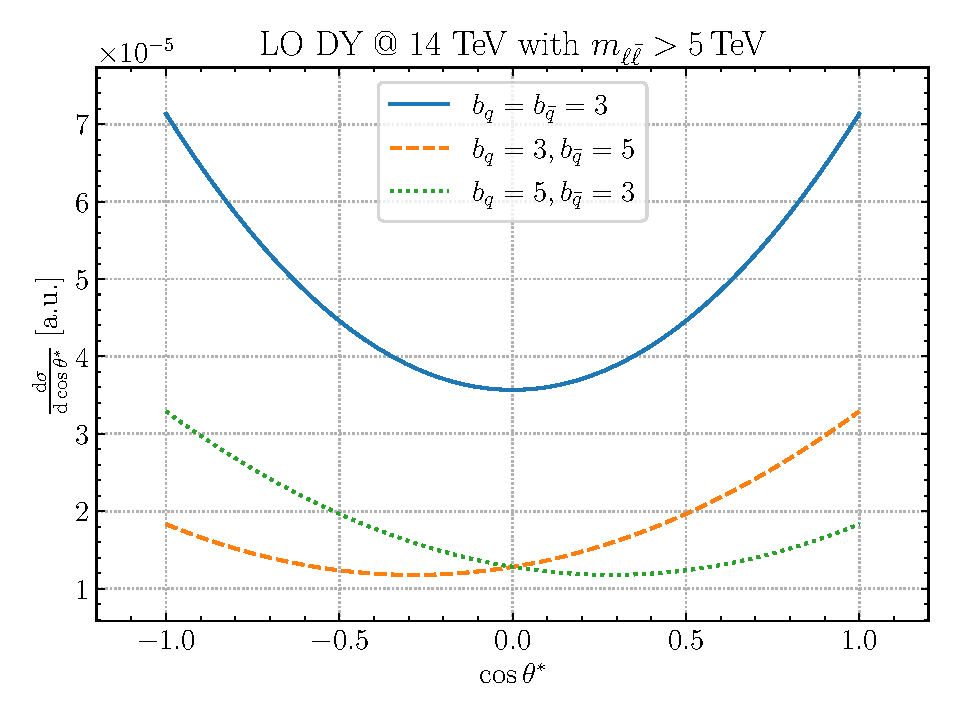
\includegraphics[width=0.49\linewidth]{ch-afb/sigma_toy-33-53-35.pdf}
 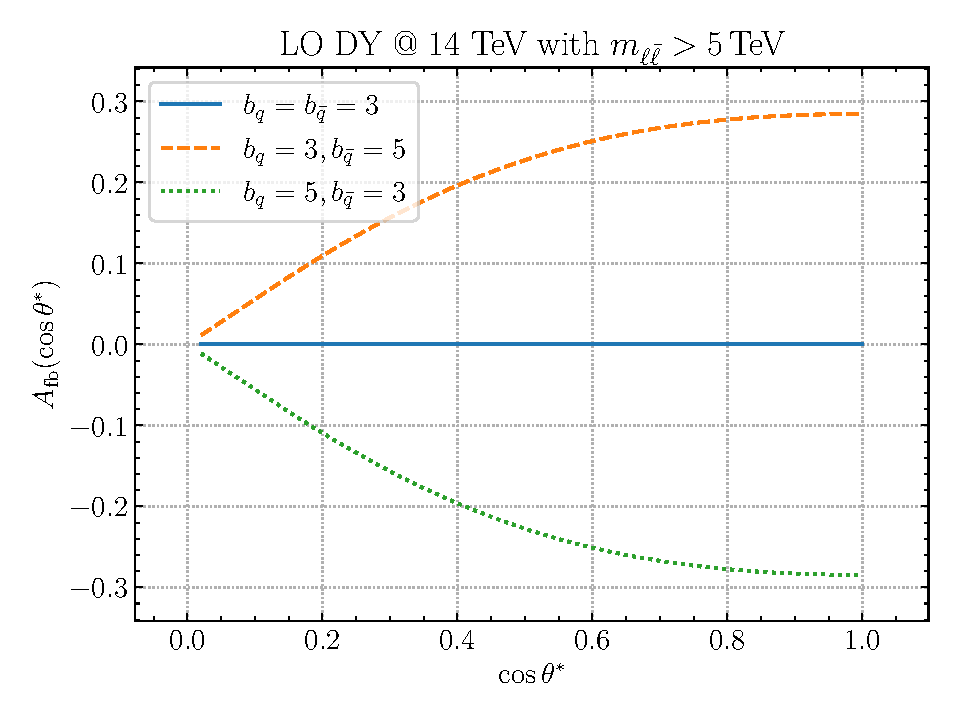
\includegraphics[width=0.49\linewidth]{ch-afb/afb_toy-33-53-35.pdf}
 \caption{The single-inclusive $\cos\theta^*$ distribution
   \cref{eq:afb/dsigma-dcos}  (left)
   and the corresponding forward-backward asymmetry
   (right panel) \cref{eq:afb/forward-backward-asymmetry} evaluated using 
    the toy \pdfs of \cref{eq:afb/toypdf}.
   %
   No  kinematic cuts are applied except for $\mll^{\text{min}}=5$ TeV.
   %
 }    
 \label{fig:afb/sigma_toy}
\end{figure}
%-----------------------------------------------------------------

In \cref{fig:afb/sigma_toy} we display both the $\cos\theta^*$
single-inclusive distribution \cref{eq:afb/dsigma-dcos} and
the asymmetry \cref{eq:afb/forward-backward-asymmetry}.
%
It is apparent that if the  antiquark \pdfs fall off at large-$x$ faster than
the quarks, i.e.\ when $b_q < b_{\bar{q}}$ the forward-backward
asymmetry is positive, while if the converse is true it is
negative. Of course if the quark and antiquark \pdfs behave in the same
way there is no asymmetry.
%
In this simple model, a negative asymmetry corresponds to a negative
valence distribution, which conflicts with sum rules and appears to be
unphysical. However, the model should be only taken as illustrative of
the large-$x$ behavior: it is of course easy to construct \pdfs that
reproduce this behavior at very large $x$, while leading to a positive
valence \pdf as $x$ decreases, consistent with sum rules. One could then argue that
Brodsky-Farrar counting rules~\cite{Brodsky:1973kr,Brodsky:1974vy}
imply that  $b_q > b_{\bar{q}}$
hence a positive asymmetry is favored.
%
However,
counting rules are supposed to only hold asymptotically, so whether
they apply in any given region of $x$ is a priori unclear.
%
It is easy
to construct generalizations of the model in which the behavior
leading to a negative asymmetry is reproduced at large enough $x$, yet
the valence \pdfs are positive at smaller $x$, and the counting rules
apply in the strict $x\to1$ limit.

In fact, whereas in the toy model a negative asymmetry is
associated with a negative valence
\cref{eq:afb/toym}, the formal condition for a negative asymmetry is
(assuming $x_1>x_2$)
\begin{equation}\label{eq:afb/signas}
   \sign\left[\mathcal{L}_{A,q}\right]=\sign\left[\frac{ f_q^+(x_2)}{
       f_q^+(x_1)}-\frac{
       f_q^-(x_2)}{f_q^-(x_1)}\right]=\sign\left[\frac{ f_q(x_2)}{
       f_q(x_1)}-\frac{f_{\bar{q}}(x_2)}{f_{\bar{q}}(x_1)}\right] \, , \quad x_1>x_2 \,.
\end{equation}
Hence what determines the sign of the antisymmetric luminosity, and thus
of the forward-backward asymmetry, is the relative rate of decrease of
the quark and antiquark, or valence and total quark \pdfs, rather than
their sign. Again, it is easy to construct generalizations of the
toy model in which the condition \cref{eq:afb/signas} still holds,  yet
the valence \pdf remains positive.

It is interesting to note that a different conclusion is reached using
an approximation to the asymmetry which is quite accurate  in the $Z$
peak region.
%
This approximation however turns out to fail at high
invariant mass.
%
Indeed, the expression \cref{eq:afb/lumisa_qpm} of the antisymmetric
luminosity in terms of the valence 
and total \pdf combinations $f_q^+$ and $f_q^-$ \pdf combinations
suggests an approximation based on the expectation
that the valence is dominant at large $x$ and the sea is dominant at
small $x$. Assuming $x_1> x_2$, one then expects that
\begin{equation}
\mathcal{L}_{A,u}(\yll,\mll) \approx\frac {1}{2} f_u^-(x_1,\mll^2)
f_{u}^+(x_2,\mll^2)   \,  \, ,\quad x_1>x_2.
\label{eq:afb/app_asym_lumi_2}
\end{equation}
This is clearly true  in the $Z$-peak region, which  motivates the suggestion
to use the measurement of $A_{\text{fb}}$ as a means to constrain the valence
quark combinations~\cite{Accomando:2019vqt}.

%-------------------------------------------------------------------------------
\begin{figure}[!t]
 \centering
 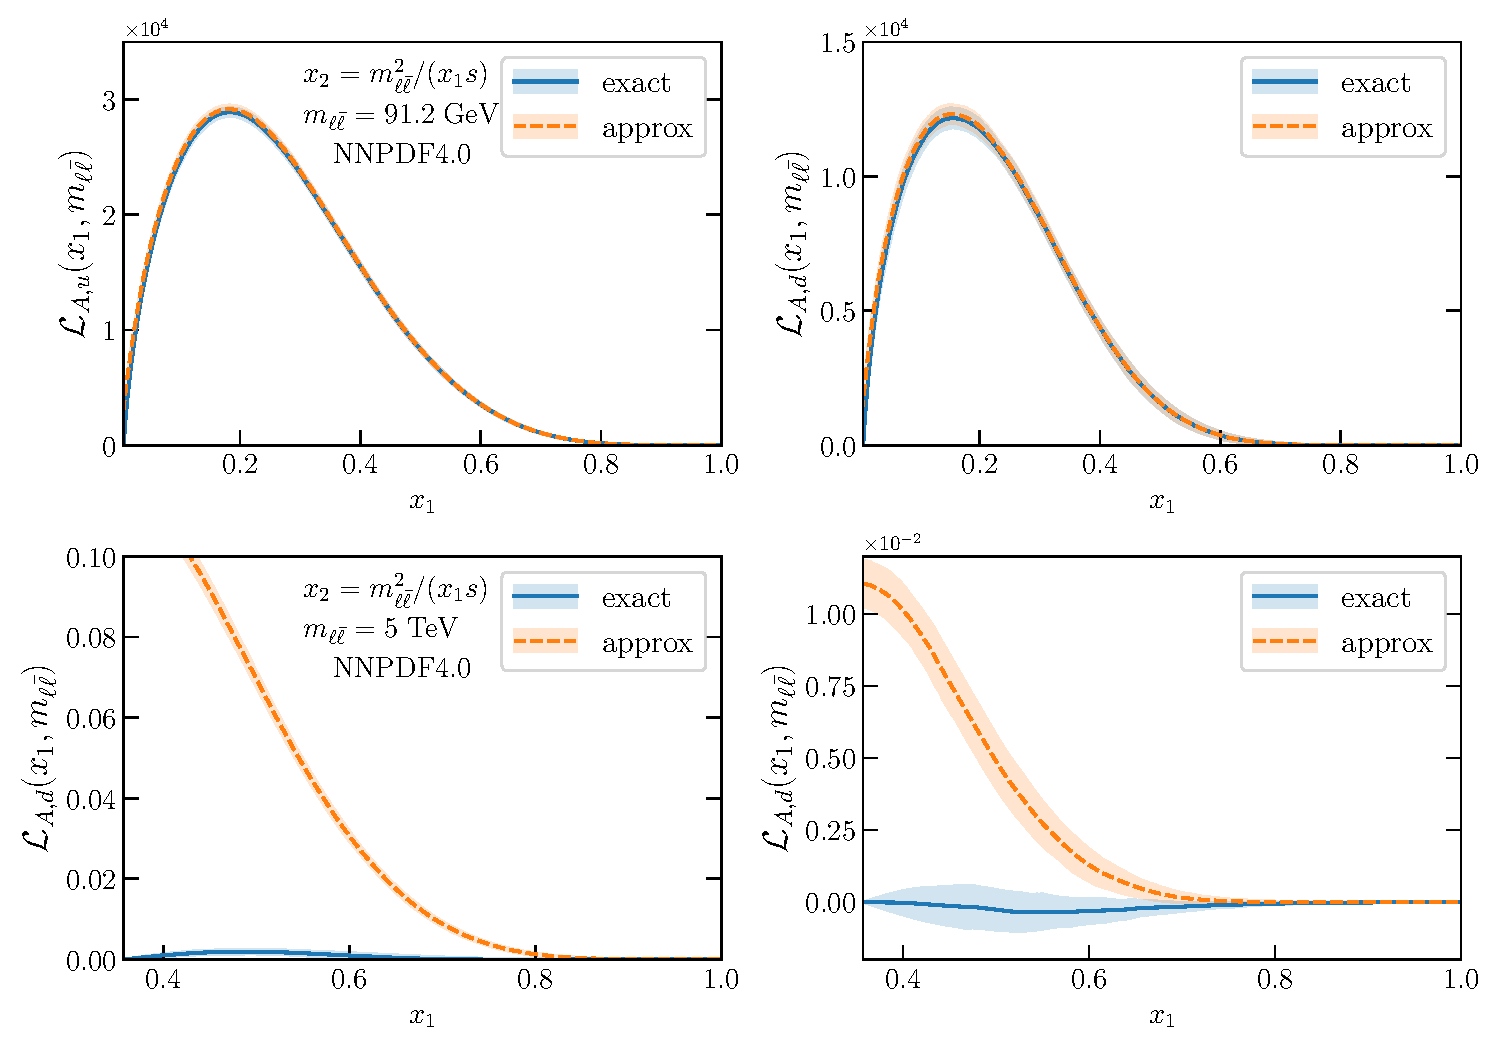
\includegraphics[width=0.90\linewidth]{ch-afb/pdfplot-abs-DYlumis-minus-validation-lowQ-nnpdf40.pdf}
 \caption{The  antisymmetric partonic luminosity $\mathcal{L}_{A,q}$, \cref{eq:afb/lumisa_qpm},
for the up and down quarks 
compared to the approximation 
\cref{eq:afb/app_asym_lumi_2} in the case of \nnpdfr{4.0}
at $\mll=m_Z$ (top)
and $\mll=5$ TeV (bottom panels).
 }    
 \label{fig:afb/pdfplot-abs-DYlumis-minus-validation-lowQ-nnpdf40}
\end{figure}
%---------------------------------------------------------------------------

However, while \cref{eq:afb/app_asym_lumi_2} provides
a satisfactory approximation in the  $Z$-peak region,
it fails  at larger $\mll$ values. Indeed, for on-shell $Z$
production, with $\sqrt{s}=14$ TeV,
for a dilepton rapidity with $y_{\ell\bar{\ell}}\sim 2.5$, the limit of the
acceptance region
of ATLAS and CMS, the colliding partons have
$x_1=0.09$ and $x_2=6\times 10^{-4}$. So indeed the contribution in
which the valence \pdf is evaluated at the smallest $x$ value is highly suppressed.
%
But for $\mll=5$~TeV, the smallest value of $x_2$, attained when
$x_1=1$, is $x_2=0.35$: so both momentum fractions are large and in fact
to the right of the valence peak.
%
In such case, there 
is no obvious hierarchy between
the different terms that contribute to to antisymmetric
luminosity $\mathcal{L}_{A,q}$.

This is illustrated in
\cref{fig:afb/pdfplot-abs-DYlumis-minus-validation-lowQ-nnpdf40},
where we compare the antisymmetric luminosity $\mathcal{L}_{A,q}$
for the up and down quarks 
to the approximation
\cref{eq:afb/app_asym_lumi_2}, evaluated with \nnpdfr{4.0} \nnlo,
in the $Z$-peak region $\mll=m_Z$ 
and at $\mll=5$ TeV.
%
While indeed for $\mll=m_Z$ \cref{eq:afb/app_asym_lumi_2} reproduces
the exact luminosity, this is not the case for $\mll\gg m_Z$: both
the magnitude and the shape of the luminosity are  very different.
%
This qualitative behavior is common to all \pdf sets: the approximation
fails equally badly regardless of the \pdf set.

We conclude that there
is no simple relation between the sign of the asymmetry and that of
the valence \pdf, and that the
behavior of the asymmetry must be determined by studying the large-$x$
behavior of the quark and antiquark \pdfs.

\subsection{Parton distributions}
\label{sec:afb/subsec-largexPDFs}

We assess now the large-$x$ behavior of
the quark and antiquark \pdfs in different recent \pdf
determinations: specifically, we compare
 ABMP16,
 CT18,  \nnpdfr{4.0},
 and MSHT20.
%
 For
completeness, in App.~\ref{app:nnpdf31} we also present results
obtained with the widely used NNPDF3.1~\cite{Ball:2017nwa} set.

%-------------------------------------------------------------------------------
\begin{figure}[!t]
 \centering
 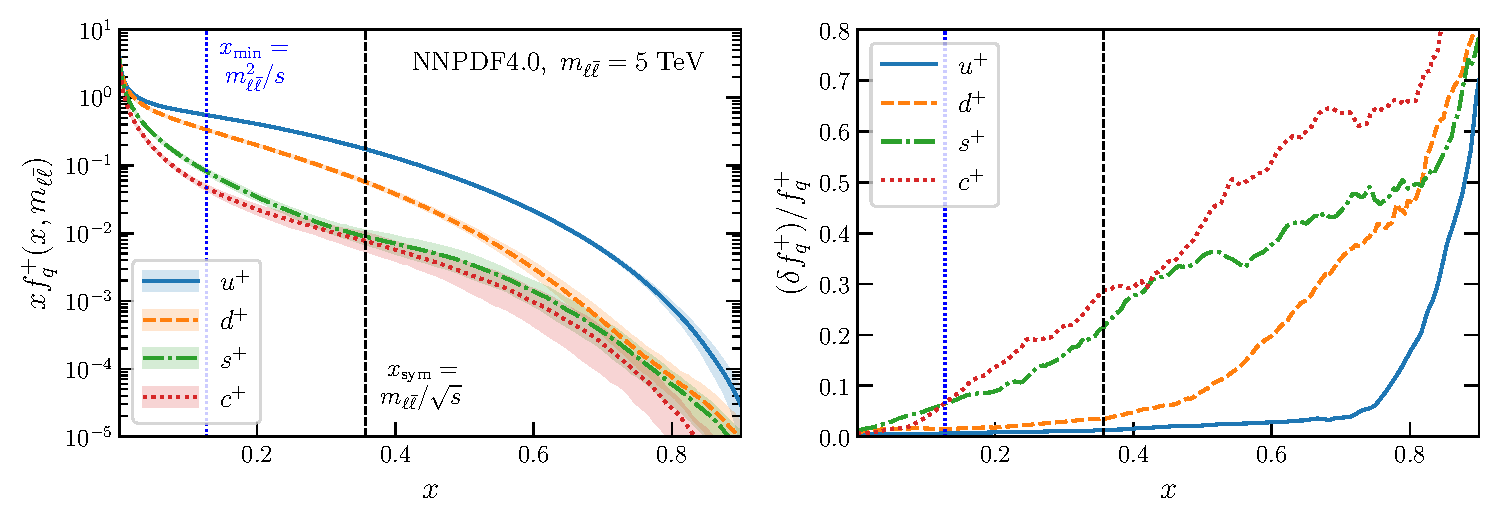
\includegraphics[width=1.0\linewidth]{ch-afb/pdfplot-abslargex-nnpdf40.pdf}
 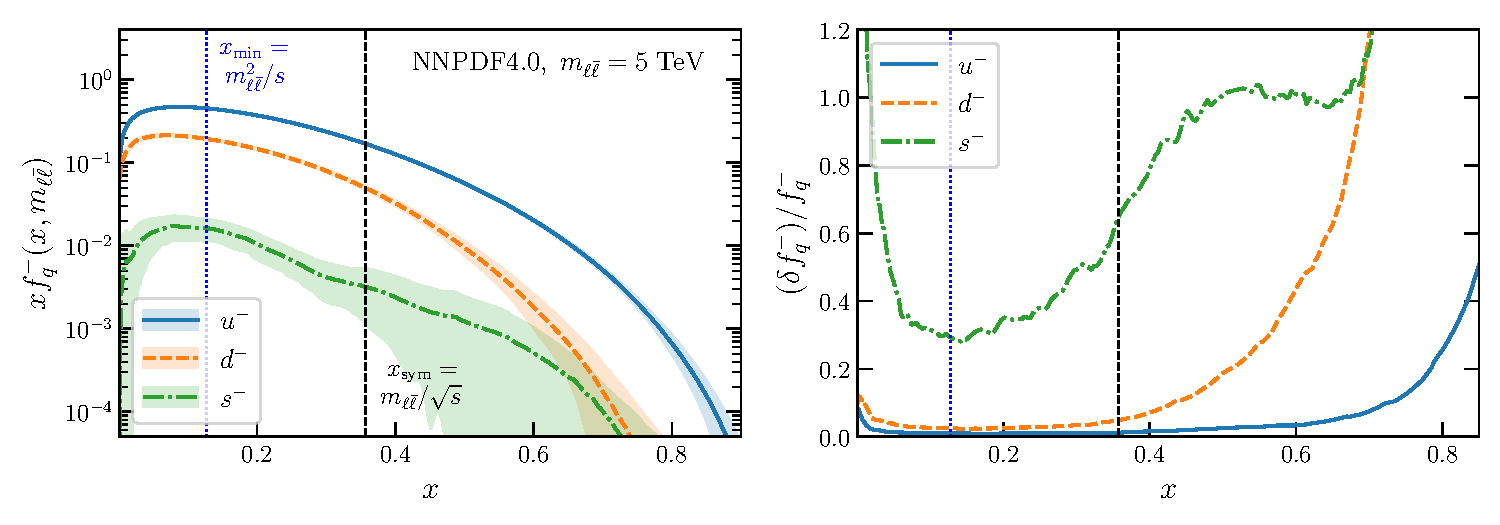
\includegraphics[width=1.0\linewidth]{ch-afb/pdfplot-abslargex-nnpdf40-valence.pdf}
 \caption{\small Comparison of the $xf^+_q$ (top) and $xf_q^-$ (bottom) quark
   \pdf combinations for the up, down, strange, and charm quarks,
   evaluated at $\mll=5$~TeV for \nnpdfr{4.0} \nnlo.
   %
   The right panels display the relative 68\% CL uncertainties.
   %
   The two vertical lines indicate $x_{\text{min}}=\mll^2/s$, the
   smallest allowed value of $x$ 
   for dilepton DY production for a collider
   CoM energy $\sqrt{s}=14$~TeV, and the value of $x$
   corresponding to a symmetric partonic collision $x_1=x_2$, namely
 $x_{\text{sym}}=\mll/\sqrt{s}$.
 }    
 \label{fig:afb/pdfplot-abslargex}
\end{figure}
%-------------------------------------------------------------------------------

First, we provide a qualitative assessment of the relative size of the
\pdfs corresponding to
individual quark flavors, both for the total and valence \pdfs.
In \cref{fig:afb/pdfplot-abslargex} we
compare  the total $xf^+_q$ and valence $xf_q^-$  quark
   \pdf combinations for the up, down, strange, and charm quarks,
   evaluated at $\mll=5$~TeV with the \nnpdfr{4.0} \nnlo \pdf set.
   %
   The right panels display the corresponding relative 68\% CL uncertainties.
   %
  The leftmost vertical line indicates $x_{\text{min}}=\mll^2/s$, the
  smallest allowed value of $x$ 
   for dilepton DY production with invariant mass $\mll=5$~TeV for a collider
   CoM energy $\sqrt{s}=14$~TeV.
   %
   The rightmost vertical line corresponds to
   the value of $x$ in a symmetric partonic collision where $x_1=x_2$, namely
   $x_{\text{sym}}\equiv\mll/\sqrt{s}$.

   From \cref{fig:afb/pdfplot-abslargex} one can observe that for
   $x\lesssim 0.3$ there is a clear hierarchy
$f_u^+>f_d^+ >f_s^+>f_c^+$, while for larger $x$ values the
   strange and charm \pdfs become of comparable magnitude.
   %
   The up and down quarks, both for $xf^+_q$ and $xf^-_q$, are significantly larger
   than the second-generation quark \pdfs until $x\simeq 0.7$, and hence dominate the
   large-$\mll$ differential distributions in Drell-Yan production.
%
\pdf uncertainties grow rapidly with $x$, reflecting the lack
of direct experimental constraints.
%
The same qualitative behavior of the lighter versus heavier flavor \pdfs
is observed for other \pdf sets.
%
Given the hierarchy $f_u^\pm, f_d^\pm \gg f_s^\pm, f_c^\pm $, in the following
we will discuss only the behavior of the first-generation quark
and antiquark \pdfs which are those relevant for the interpretation
of neutral-current Drell-Yan production in the kinematic region used
for \bsm searches. 
      


%---------------------------------------------------------------------------
\begin{figure}[!t]
 \centering
 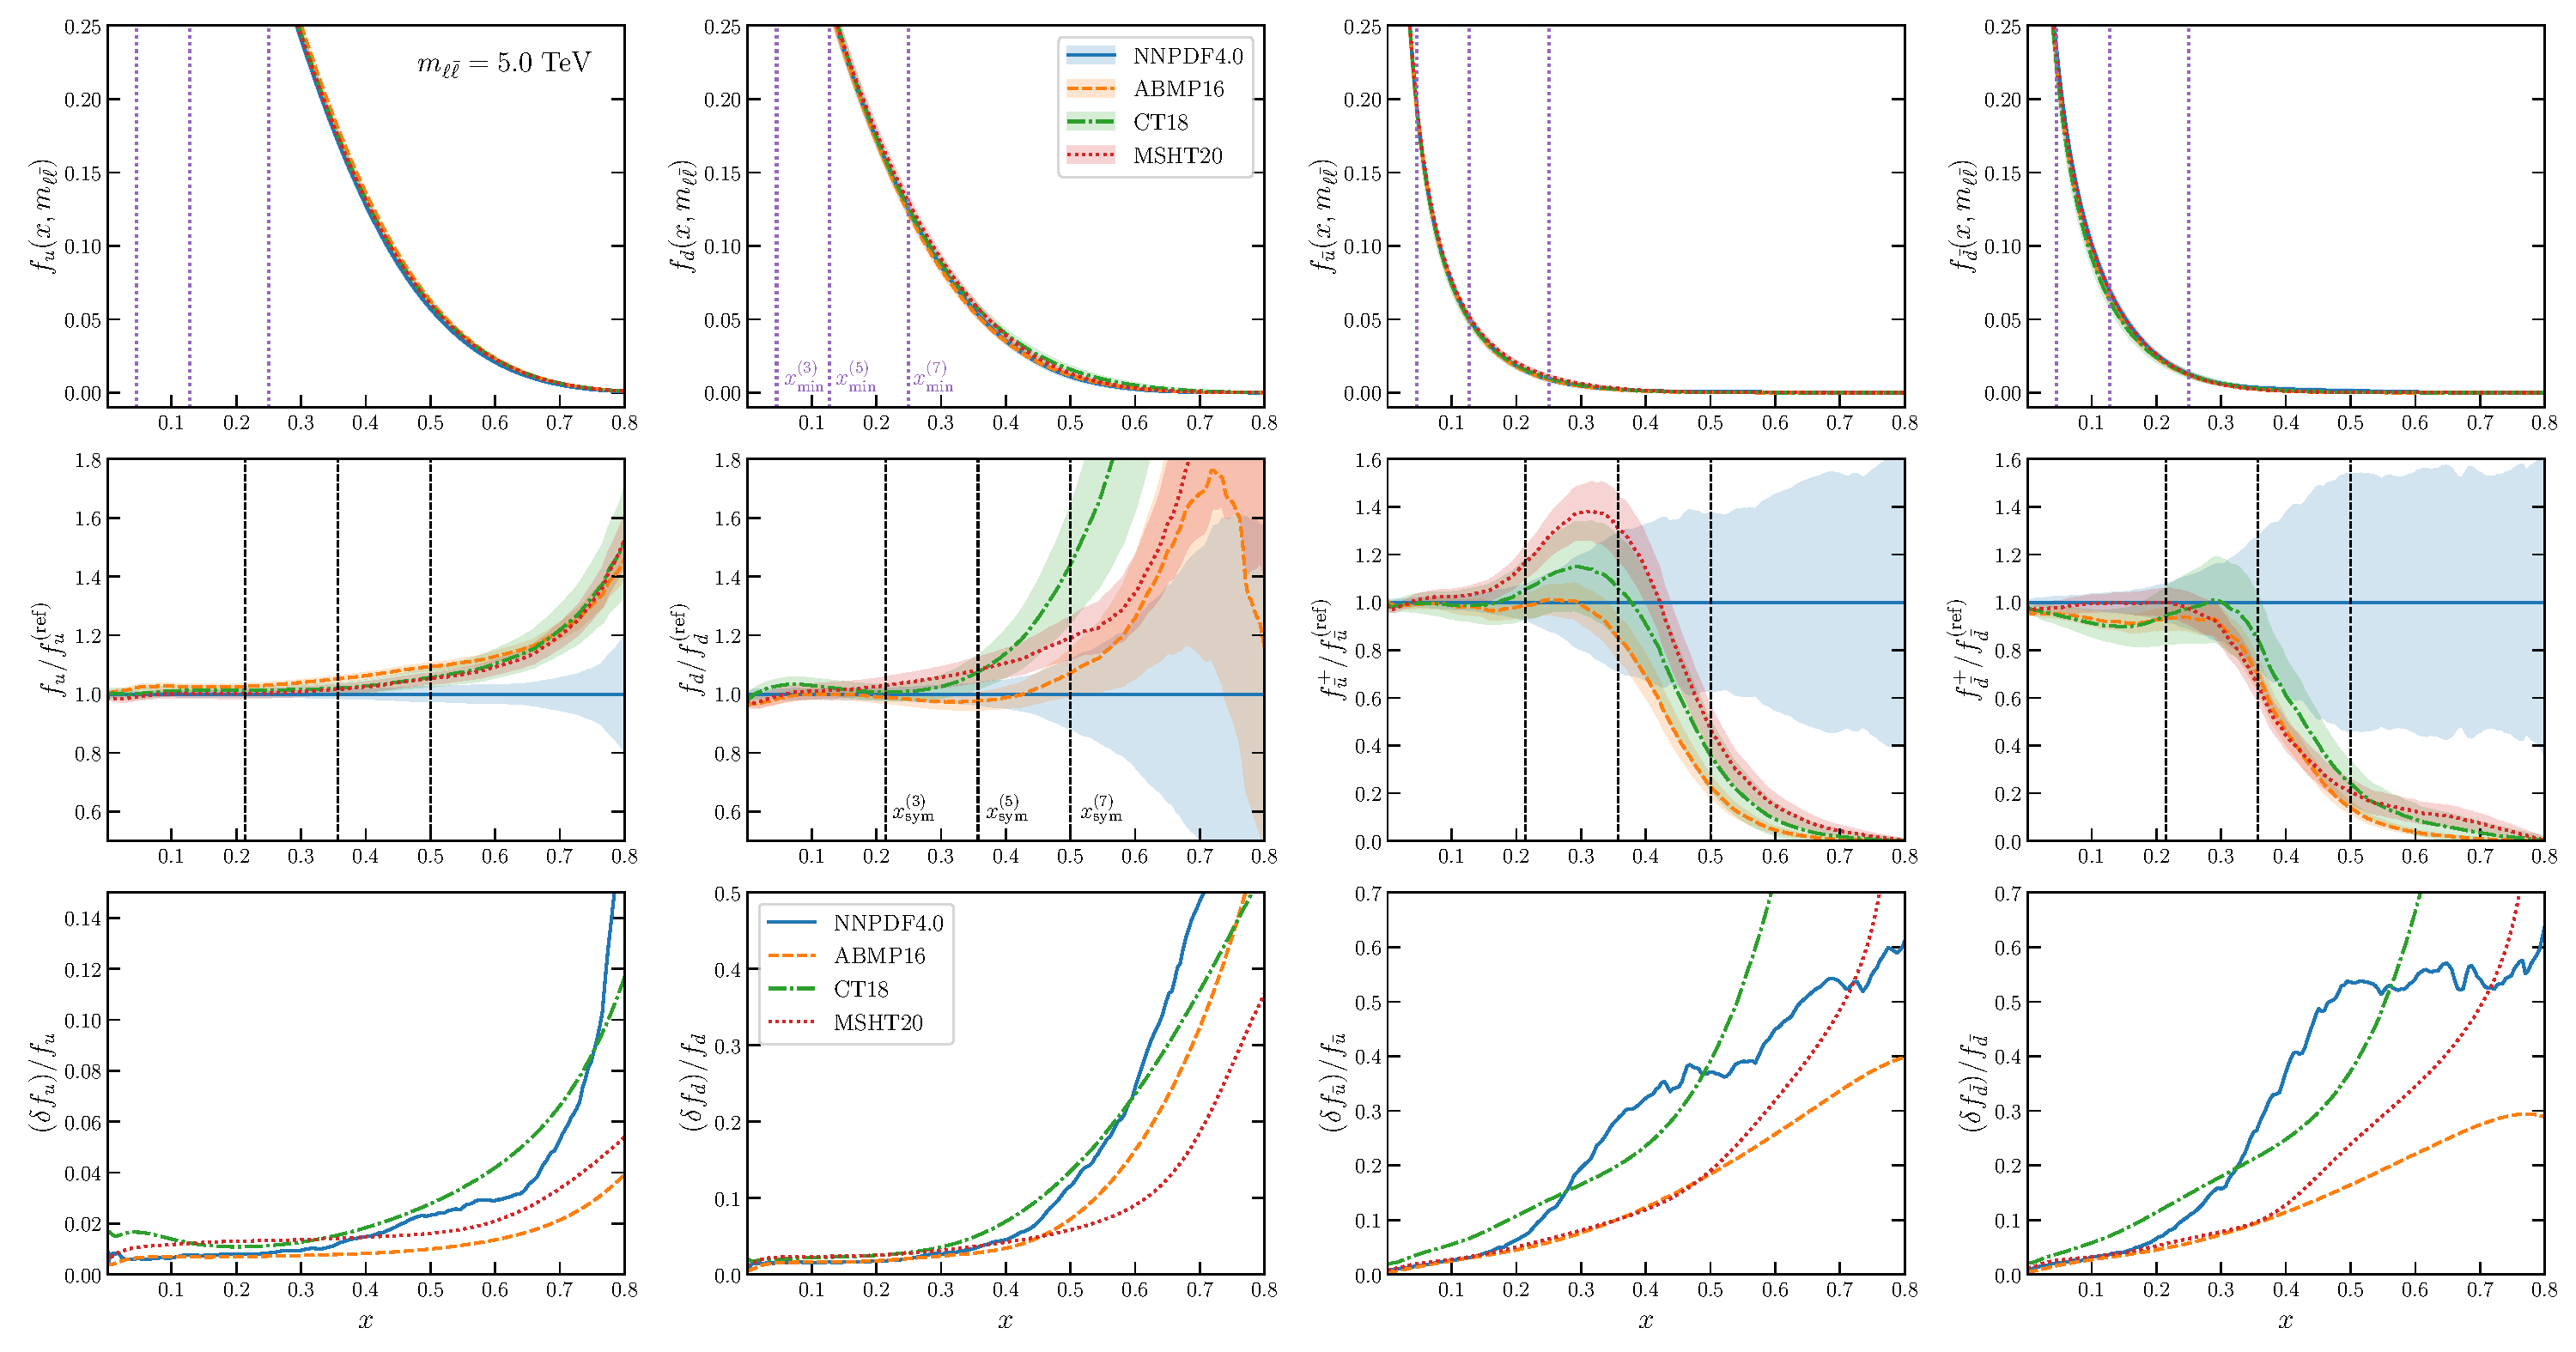
\includegraphics[width=1.00\linewidth]{ch-afb/pdfplot-pdfsets-quarks-antiquarks-q5p0tev.pdf}
 \caption{\small The up and down quark and antiquark \pdfs evaluated at $\mll=5$ TeV
   for \nnpdfr{4.0}, CT18, MSHT20, and ABMP16 in the $x$ region relevant for
   high-mass Drell-Yan production. The upper panels display the absolute \pdfs,
   the middle ones their ratio to the central \nnpdfr{4.0} value, and the bottom panels
   the relative 68\% CL uncertainties.
   %
   The vertical lines in the top
   row indicate the values of  $x_{\text{min}}=\mll^2/s$ and in the central
   row those of $x_{\text{sym}}=\mll/\sqrt{s}$
   for three
   different values  $\mll=3,\,5,\,7$~TeV.
   %
   Note that in the second row the
   range on the $y$ axis is not the same for quarks and antiquarks,
   and in the third row also for up and down quarks.
   %
   Note also that the
   \pdfs, their ratios and their uncertainties are essentially
   unchanged in the displayed large-$x$ region in the range $1~{\text{TeV}}<\mll<7$~TeV.
}    
 \label{fig:afb/mll_dep_pdfs}
\end{figure}
%---------------------------------------------------------------------------

We next compare the large-$x$ behavior 
of the four \pdf sets ABMP16, CT18, MSHT20, and \nnpdfr{4.0} in \cref{fig:afb/mll_dep_pdfs}
for $\mll=5$~TeV.
%
We display from top to bottom the absolute \pdfs, their ratio to the central \nnpdfr{4.0} value, and
their relative 68\% CL uncertainties.
%
As in the case of \cref{fig:afb/pdfplot-abslargex}, we indicate with two vertical lines
the values of $x_{\text{min}}$ and $x_{\text{sym}}$,
both for $\mll=5$~TeV, and for a smaller and a larger value of $\mll$,
namely for $\mll=3$~TeV and  $\mll=7$~TeV.
%
For clarity, the values of $x_{\text{min}}$ are only shown 
in the top row of plots, and the values of  $x_{\text{sym}}$ in the
central row. Note that the scale dependence
of the \pdfs in this range of  $x$ and invariant mass is very
slight. Indeed, the \pdfs shown in \cref{fig:afb/pdfplot-abslargex} are
essentially unchanged at $\mll=3$ TeV or  $\mll=7$ TeV;  only the
corresponding ranges of $x_1$, $x_2$ vary significantly.

Good agreement between all \pdf
sets is found up to around $x\simeq 0.4$.
%
For $\mll=5$~TeV this corresponds to the value of $x_{\text{sym}}$, i.e.\ central rapidity.
%
For larger values of $x\gsim 0.4$, the up  quark \pdf $xf_u$ from the
\nnpdfr{4.0} set is somewhat
suppressed in comparison to the other three sets, which in turn agree
among each other.
%
A rather stronger suppression of
\nnpdfr{4.0}  in comparison to  CT18 is observed for the down quark, with
MSHT20 and ABMP16 in a somewhat intermediate situation.
%
The opposite behavior is found in the same region $x\gsim 0.4$ for
antiquark \pdfs  $xf_{\bar{u}}$ and $xf_{\bar{d}}$:
namely, the \nnpdfr{4.0} \pdf is significantly  larger than that of the other sets.
It follows that for a lower invariant mass value  $\mll = 3$~TeV, all
\pdf sets are  in agreement in the $x$ range in which they are probed,
while for a higher value  $\mll = 7$~TeV the 
disagreement between \nnpdfr{4.0} and the other \pdf sets is present for
most of the $x\ge x_{\text{min}}$ range.

It is interesting to observe that in the region with $0.4\lesssim x\lesssim
0.6$ the \pdfs are constrained by some fixed-target DIS structure functions and
by forward $W$ and $Z$ production data from \lhcb.
Hence, at the edge of the data region \nnpdfr{4.0} starts disagreeing with the
other global \pdf sets considered here, with the disagreement getting more
marked as $x$ grows outside the region covered by the data.
%
Qualitatively, \nnpdfr{4.0} is characterized by the fact that the
quark \pdfs drop faster as a function of $x$, and the antiquark \pdfs
drop less fast as $x$ grows towards $x=1$.
As we will show next, this feature will lead to significant differences
in the antisymmetric \pdf luminosities $\mathcal{L}_{A,q}$ as the value of
the dilepton invariant mass $\mll$ is increased.

The relative \pdfs uncertainties, shown in the lower panels in
\cref{fig:afb/mll_dep_pdfs} in all cases grow with $x$ (see also 
\cref{fig:afb/pdfplot-abslargex}).
%
The largest \pdf uncertainties correspond to either CT18 or \nnpdfr{4.0}, 
depending on the $x$ range and the \pdf flavor.
%
Specifically, the \nnpdfr{4.0} uncertainties are largest for $f_d$ in the
region $x\gsim 0.6$ 
and for $f_{\bar{u}}$ and $f_{\bar{d}}$ when $0.3 \lsim x \lsim 0.5$.
%
The smallest \pdf uncertainties are displayed by ABMP16 and  MSHT20.

The different behavior of the rate of decrease with $x$ of
\pdfs  in the large $x$ region, specifically comparing \nnpdfr{4.0}
to other \pdf sets, can  be seen most clearly from a comparison off
effective asymptotic exponents~\cite{Ball:2016spl}
\begin{equation}
  \beta_{a,q}(x,Q)\equiv\frac{\partial \ln|xf_q(x,Q)|}{\partial \ln(1-x)}\,,
  \label{eq:afb/beta_asy}
\end{equation}
which of course for \pdfs of the form of \cref{eq:afb/toypdf} just
coincide with the exponent $b$ up to $O(1-x)$ corrections.
In \cref{fig:afb/asy_exponents} we compare
the values of $\beta_{a,q}(x,\mll)$
for ABMP16, CT18, MSHT20, and \nnpdfr{4.0} evaluated at $\mll=5$~TeV
for the up and down quark and antiquark \pdfs in the  $x$ range of
\cref{fig:afb/pdfplot-abslargex}.

It is clear that while all \pdf
sets have a similar effective asymptotic exponent for $x\lsim 0.35$, a
different behavior of \nnpdfr{4.0} in comparison to other
determinations sets in for $x\gsim 0.4$.
%
Specifically, for quarks the \nnpdfr{4.0} exponents are always larger,
and for antiquarks smaller than those found with other \pdf
sets.
%
Interestingly, whereas for the up quark the
effective exponent $\beta_{a,u}$ is approximately constant for all
\pdf sets when  $x\gsim 0.4$, with the \nnpdfr{4.0} value being just
slightly higher and slowly increasing, for the down quark and all
antiquarks this approximately constant behavior is seen for other
\pdf sets but not for \nnpdfr{4.0}.
%
Specifically, for the \nnpdfr{4.0} down quark
the exponent slowly but markedly increases for $x\gsim 0.3$, together 
with its uncertainty.
%
In the case of \nnpdfr{4.0} for both antiquarks the exponent
rapidly drops  in the region $0.3 \lsim x \lsim 0.4$.
%
This is consistent with the observation at the \pdf level
(\cref{fig:afb/mll_dep_pdfs})  that for \nnpdfr{4.0}
at large-$x$, as compared to the other groups,
the up and especially the down  quark fall off more rapidly, while
the antiquark \pdfs drop more slowly. Note in particular that for
the down \pdf the antiquark effective exponent is significantly
smaller than the quark effective exponent for all $x\gsim0.4$.

%-------------------------------------------------------------------------------
\begin{figure}[!t]
 \centering
 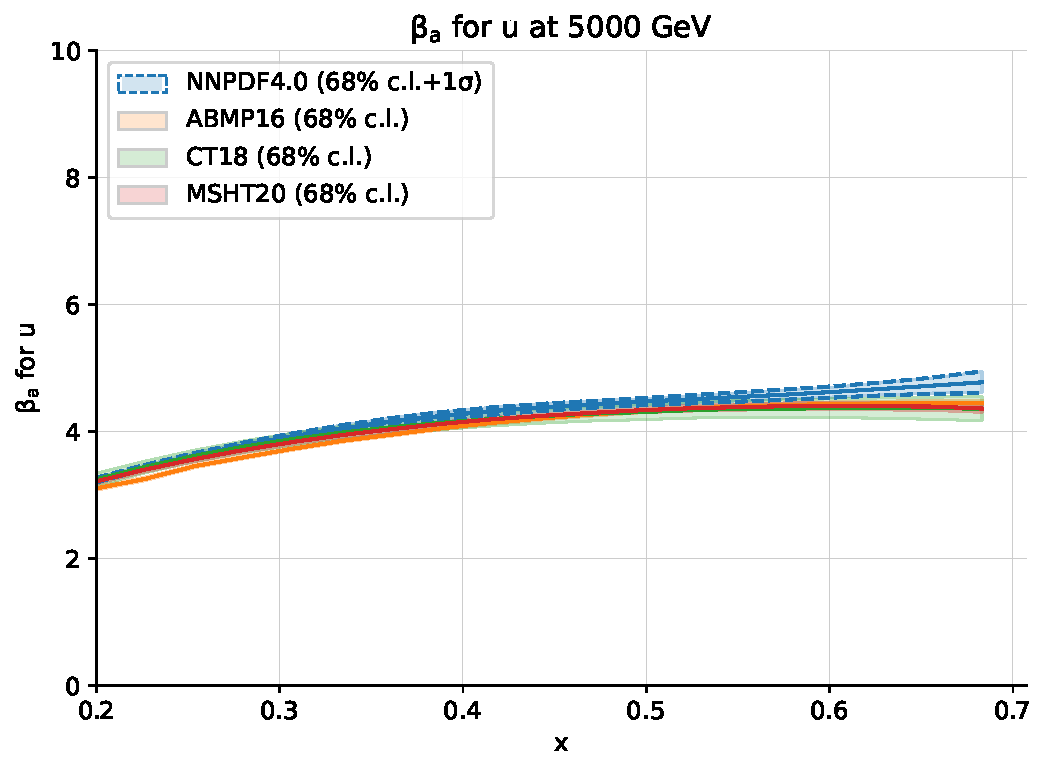
\includegraphics[width=0.49\linewidth]{ch-afb/beta_q_plot_beta_asy_u.pdf}
 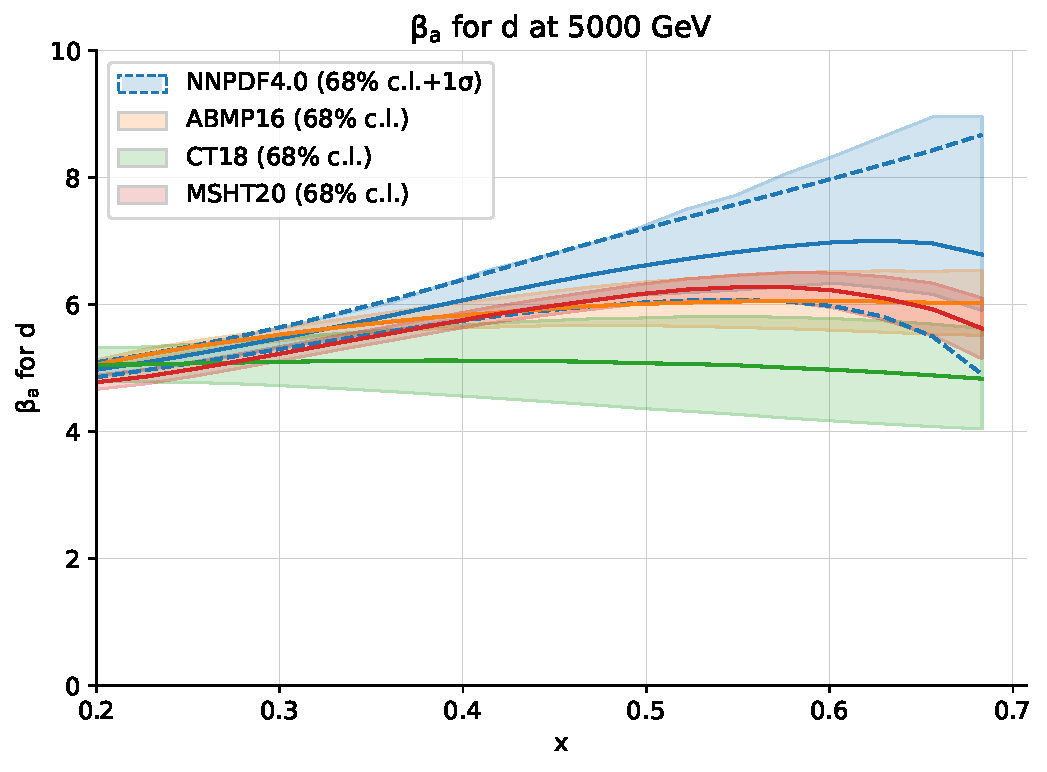
\includegraphics[width=0.49\linewidth]{ch-afb/beta_q_plot_beta_asy_d.pdf}
 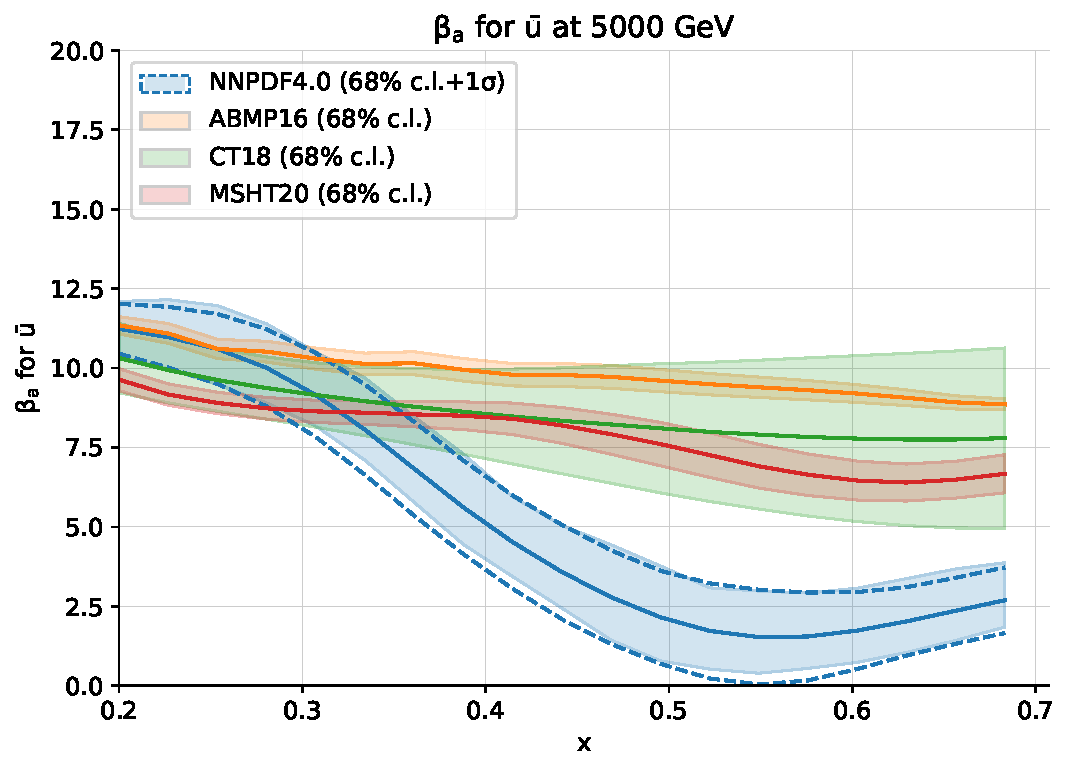
\includegraphics[width=0.49\linewidth]{ch-afb/beta_qbar_plot_beta_asy_baru.pdf}
 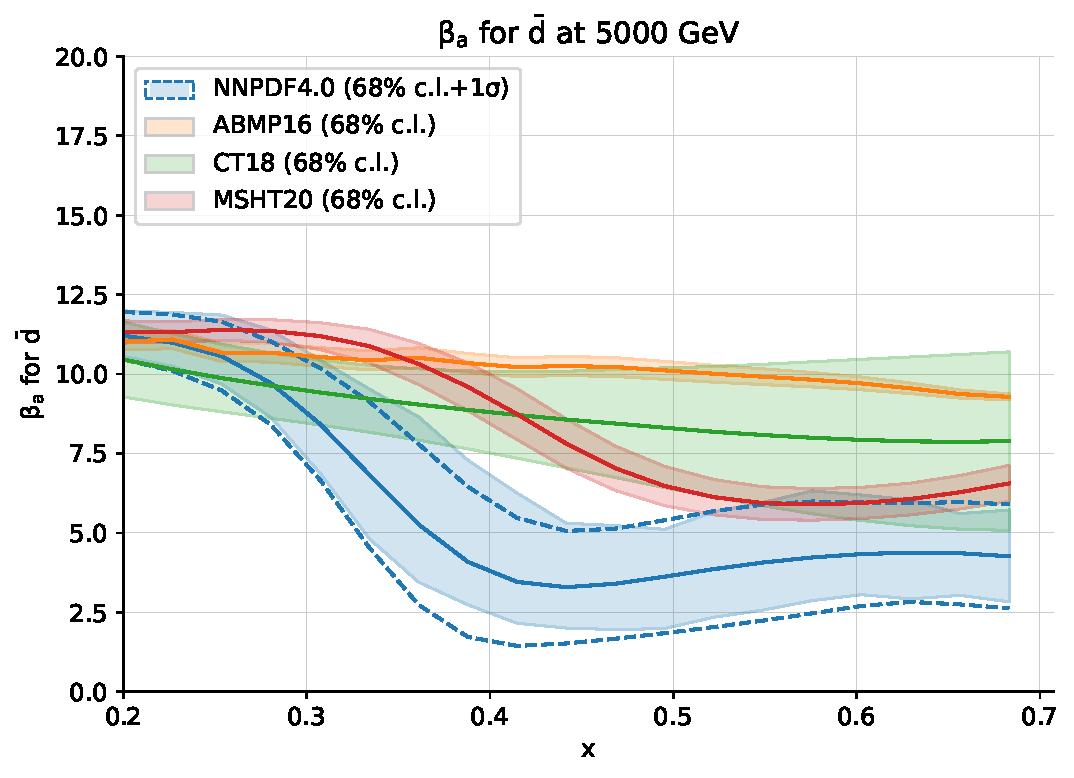
\includegraphics[width=0.49\linewidth]{ch-afb/beta_qbar_plot_beta_asy_bard.pdf}
 \caption{\small 
   The large-$x$ asymptotic exponents $\beta_{a,q}(x,\mll)$, defined in
   \cref{eq:afb/beta_asy}, for ABMP16, CT18, MSHT20, and \nnpdfr{4.0} evaluated at
   $\mll=5$~TeV for the up and down quark and antiquark \pdfs.
 }
 \label{fig:afb/asy_exponents}
\end{figure}
%-------------------------------------------------------------------------------

The fact that a modification in behavior of the effective down quark
and especially antiquark \pdfs is observed at the edge of the data
region for \nnpdfr{4.0}, but not for other \pdf sets, suggests that this
might be related to the fact that  \nnpdfr{4.0} generally adopts a more
flexible \pdf parametrization in comparison to other groups.
%
Also, the  uncertainties on the effective exponents
$\beta_{a,q}(x,\mll)$ tend to be larger for \nnpdfr{4.0} (and also to a
lesser extent for CT18) in comparison to those of other groups.
Note however that the full \pdf uncertainty contains also a
contribution from the overall 
magnitude, which is not captured by the effective exponents displayed here.

\subsection{Parton luminosities}
\label{subsec:afb/partoniclumis}

We finally turn to the behavior of parton luminosities, with
particular regard for the antisymmetric combination which is relevant
for the forward-backward asymmetry.
As for \pdfs, we first assess the qualitative features of the
luminosities corresponding to different quark flavors.
Specifically, the symmetric $\mathcal{L}_{S,q}$ and antisymmetric
$\mathcal{L}_{A,q}$ luminosities
\cref{eq:afb/symm_asymm_lumis}  for individual flavors are
displayed in \cref{fig:afb/pdfplot-absDYlumis-plus-nnpdf40},
evaluated with \nnpdfr{4.0} \nnlo for $\mll=5$ TeV and $\sqrt{s}=14$ TeV.
%
The left panels display the absolute luminosities (in logarithmic and
linear scale respectively
for the $y$ and $x$ axes)
while the right panels show the corresponding \pdf uncertainties (relative and absolute for
$\mathcal{L}_{S,q}$ and $\mathcal{L}_{A,q}$, respectively).
%
The bottom  and top $x$-axes in each plot show respectively the values
of $x_1$ and $x_2$  at which the
luminosities are being evaluated, within the allowed range
$x \ge x_{\text{sym}}=\mll/\sqrt{s}$, with the convention $x_1>x_2$.

%-------------------------------------------------------------------------------
\begin{figure}[!t]
 \centering
 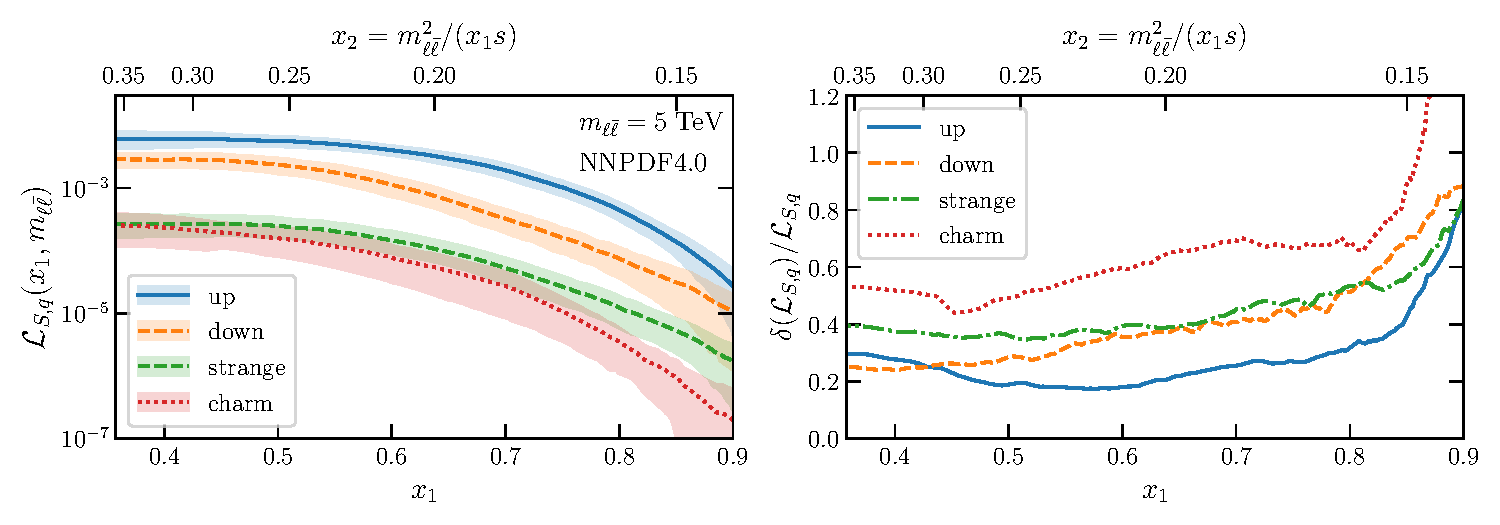
\includegraphics[width=\linewidth]{ch-afb/pdfplot-absDYlumis-plus-nnpdf40.pdf}
 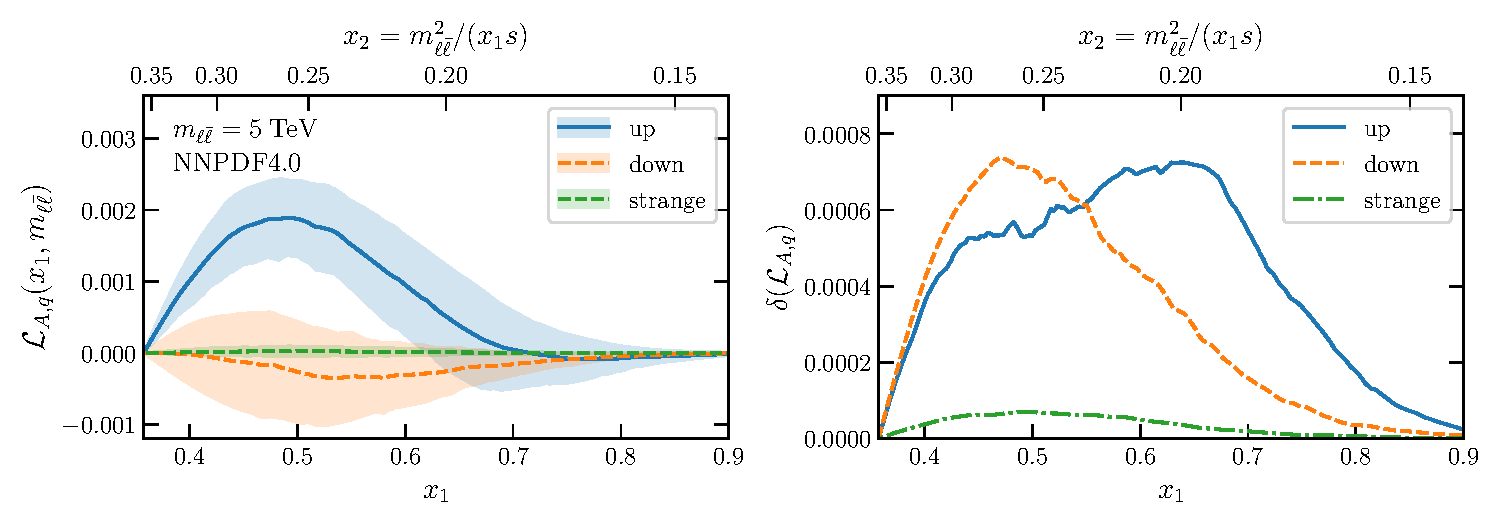
\includegraphics[width=\linewidth]{ch-afb/pdfplot-absDYlumis-minus-nnpdf40.pdf}
 \caption{The symmetric $\mathcal{L}_{S,q}$ (top)
   and antisymmetric $\mathcal{L}_{A,q}$ (bottom)
   parton
   luminosities (left) and relative uncertainties (right) evaluated with
   \nnpdfr{4.0} \nnlo at $\mll=5$ TeV and $\sqrt{s}=14$ TeV.
   %
The bottom  and top $x$-axes in each plot show respectively the values
of $x_1$ and $x_2$  at which the
luminosities are being evaluated, within the allowed range
$x \ge x_{\text{sym}}=\mll/\sqrt{s}$, with the convention $x_1>x_2$.}    
 \label{fig:afb/pdfplot-absDYlumis-plus-nnpdf40}
\end{figure}
%---------------------------------------------------------------------------

The symmetric parton luminosities exhibit of course the same hierarchy
between flavors
as the corresponding \pdf plots of \cref{fig:afb/pdfplot-abslargex}. 
%
The luminosity $\mathcal{L}_{S,q}$  drops rapidly for
$x_1\gsim 0.6$. \pdf  uncertainties  depend weakly on  $x$
up to $x_1\gsim 0.8$, after which they blow up, and range between $\sim 20\%$
for the up quark luminosity to $\sim 60\%$ for the charm quark one,
with down and strange intermediate and of similar magnitude.

As displayed in \cref{fig:afb/mll_dep_lumi_plus}, the light quark symmetric luminosities of other global \pdf sets
are qualitatively similar.
%
We show $\mathcal{L}_{S,u}$,  $\mathcal{L}_{S,d}$,
and their weighted sum that enters the  enters the
symmetric coefficient $g_{S,q}$ in \cref{eq:afb/dsigma-dcos-v2}
for the \nnpdfr{4.0}, ABMP16,
CT18, and MSHT20 at $\mll=5$ TeV.
%
The luminosities are multiplied by the effective charges
$S_q$ defined in \cref{eq:afb/coup},
and the bottom panels display the corresponding 68\% CL \pdf uncertainties.
%
Good agreement between the four sets, with a similar shape
of $\mathcal{L}_{S,q}$, is observed.
%
The \pdf luminosities for the dominant $\mathcal{L}_{S,u}$ contribution are the largest for \nnpdfr{4.0}.

%-------------------------------------------------------------------------------
\begin{figure}[!t]
 \centering
 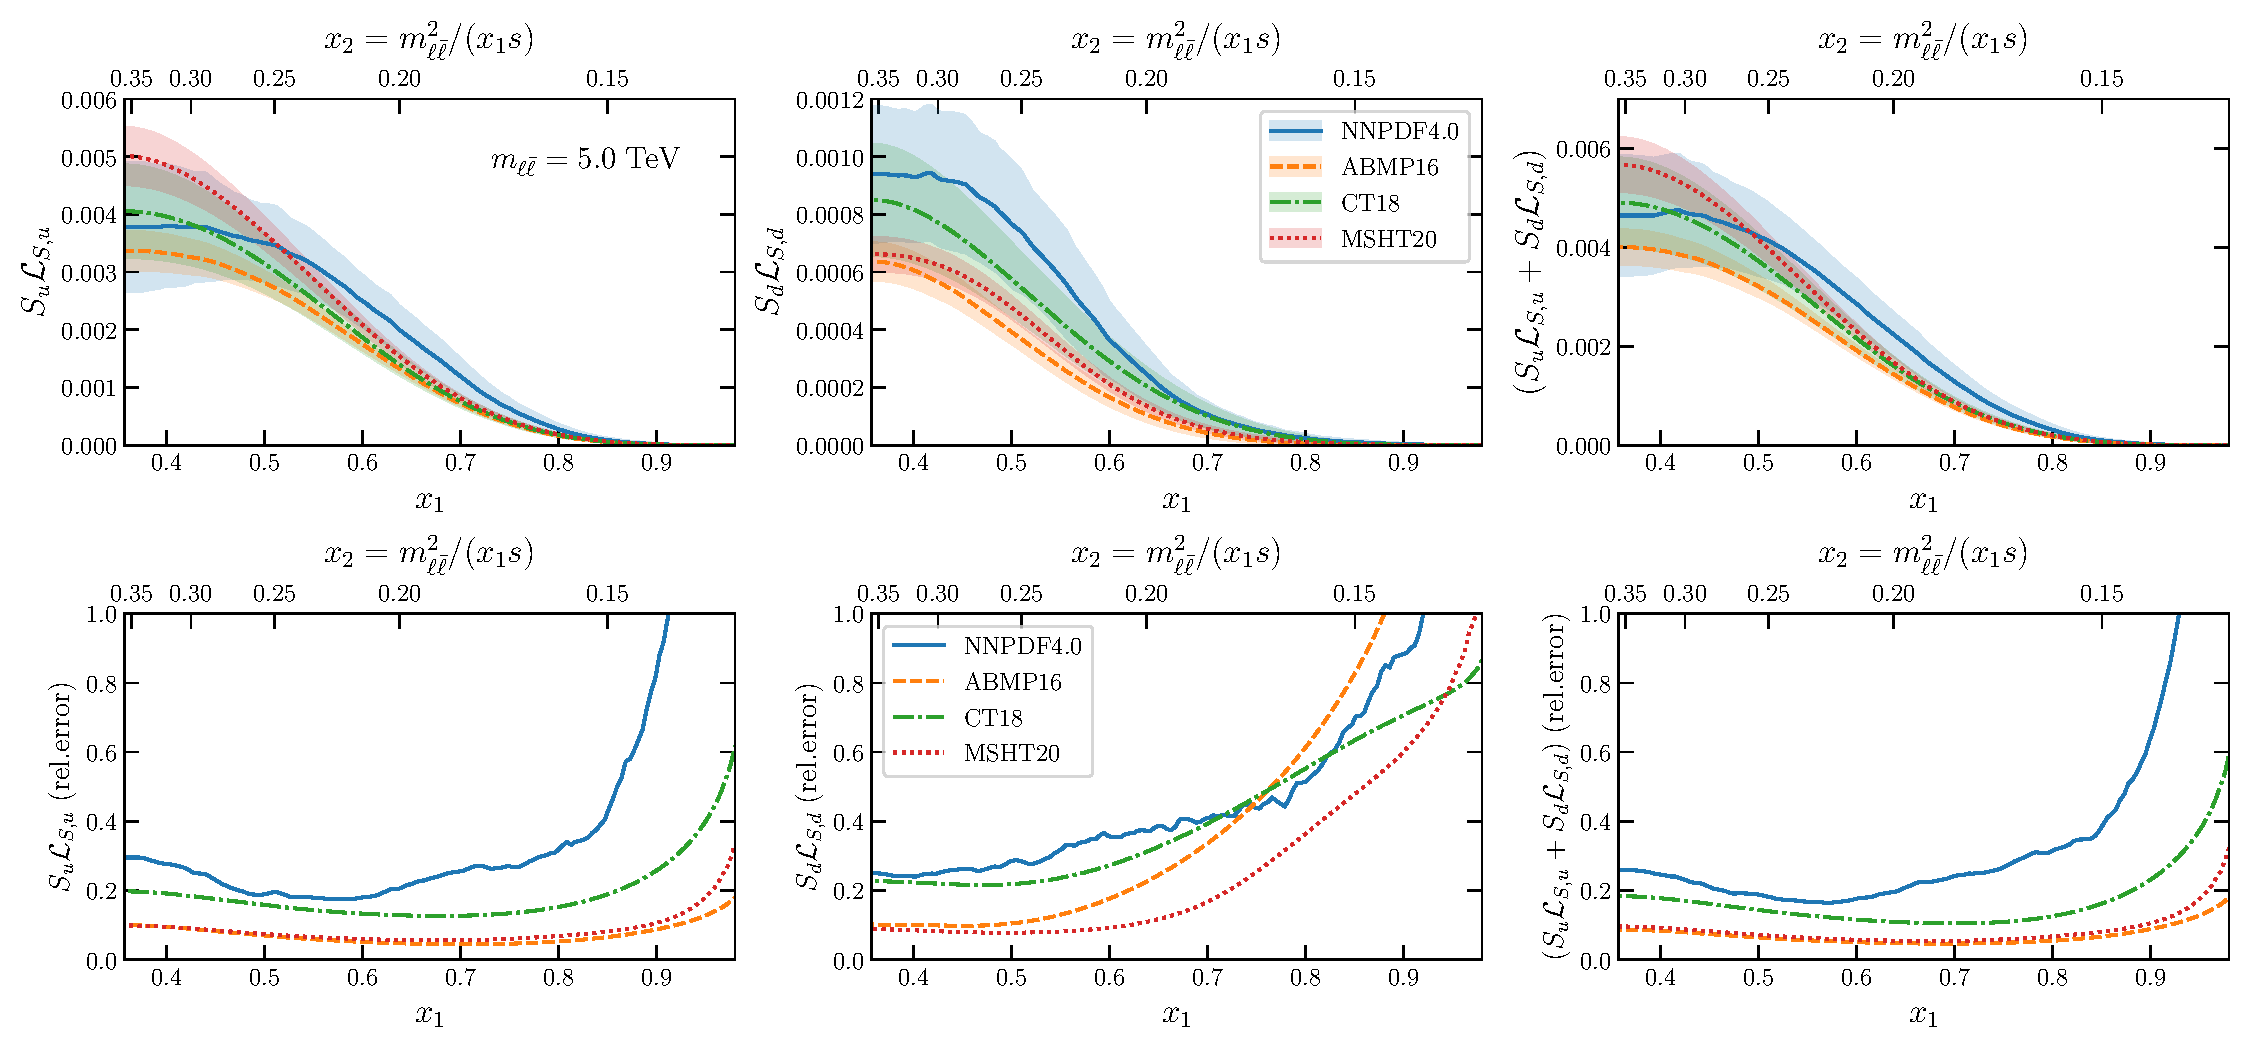
\includegraphics[width=1.00\linewidth]{ch-afb/pdfplot-abs-jacobian-DYlumis-pdfsets-plus-q5p0tev.pdf}
  \caption{The symmetric 
   parton luminosities $\mathcal{L}_{S,q}(x_1,\mll)$ for the \nnpdfr{4.0}, ABMP16,
   CT18, and MSHT20 \nnlo \pdf sets for dilepton
   invariant masses of $\mll=5$ TeV.
   %
   The luminosities are multiplied by the effective charges
   $S_q$ defined in \cref{eq:afb/coup}.
   %
   From left to right, we display $\mathcal{L}_{S,u}$,  $\mathcal{L}_{S,d}$,
   and their weighted sum that enters the  coefficient $g_{S,q}$ in \cref{eq:afb/dsigma-dcos-v2}.
   %
   The bottom panels display the relative 68\% CL \pdf uncertainties.
    }    
 \label{fig:afb/mll_dep_lumi_plus}
\end{figure}
%---------------------------------------------------------------------------

Turning to the antisymmetric \pdf luminosities $\mathcal{L}_{A,q}$,
we note  that, for \nnpdfr{4.0}, while the up luminosity is
positive, the central value of the down luminosity is negative, though
the luminosity is compatible with zero at the one sigma level.
%
Recalling
from \cref{fig:afb/pdfplot-abslargex} that $xf_{d}^-$ itself is
positive for all values of $x$,  this provides an explicit example in
which the condition \cref{eq:afb/signas} is satisfied without the valence
combination being negative.
%
We conclude that for \nnpdfr{4.0}, the faster
drop of the quark distribution and slower drop of the antiquark
distribution that was displayed by the effective exponents of
\cref{fig:afb/asy_exponents} leads to a negative antisymmetric
luminosity, in agreement with \cref{eq:afb/signas}.
The absolute \pdf uncertainties are of a similar size for
$\mathcal{L}_{A,u}$ and $\mathcal{L}_{A,d}$, with a different shape
reflecting the underlying central values.

We compare
in \cref{fig:afb/mll_dep_lumi_minus}
the behavior of the antisymmetric luminosities for all \pdf
sets for $\mll=3$ TeV (top) and $\mll=5$ TeV (bottom).
%
In order to facilitate the understanding of the way the \pdf behavior
determines that of the asymmetry, we show both the contribution of
individual flavors and the total contribution
to the antisymmetric coefficient $g_{A,q}$ of
\cref{eq:afb/gAq_integrated_1}. Namely, in
\cref{fig:afb/mll_dep_lumi_minus} the luminosities corresponding to
individual flavors are multiplied by the corresponding flavor-dependent
effective charges $A_q$ defined in \cref{eq:afb/coup}:
from left to right we display $\mathcal{L}_{A,u}$,  $\mathcal{L}_{A,d}$,
and their weighted sum
 which determines
the sign and magnitude of the total forward-backward asymmetry.
%
The corresponding absolute \pdf uncertainties for each of the four \pdf sets
are displayed in  \cref{fig:afb/mll_dep_lumi_minus_pdferrs}.

%-------------------------------------------------------------------------------
\begin{figure}[!t]
 \centering
 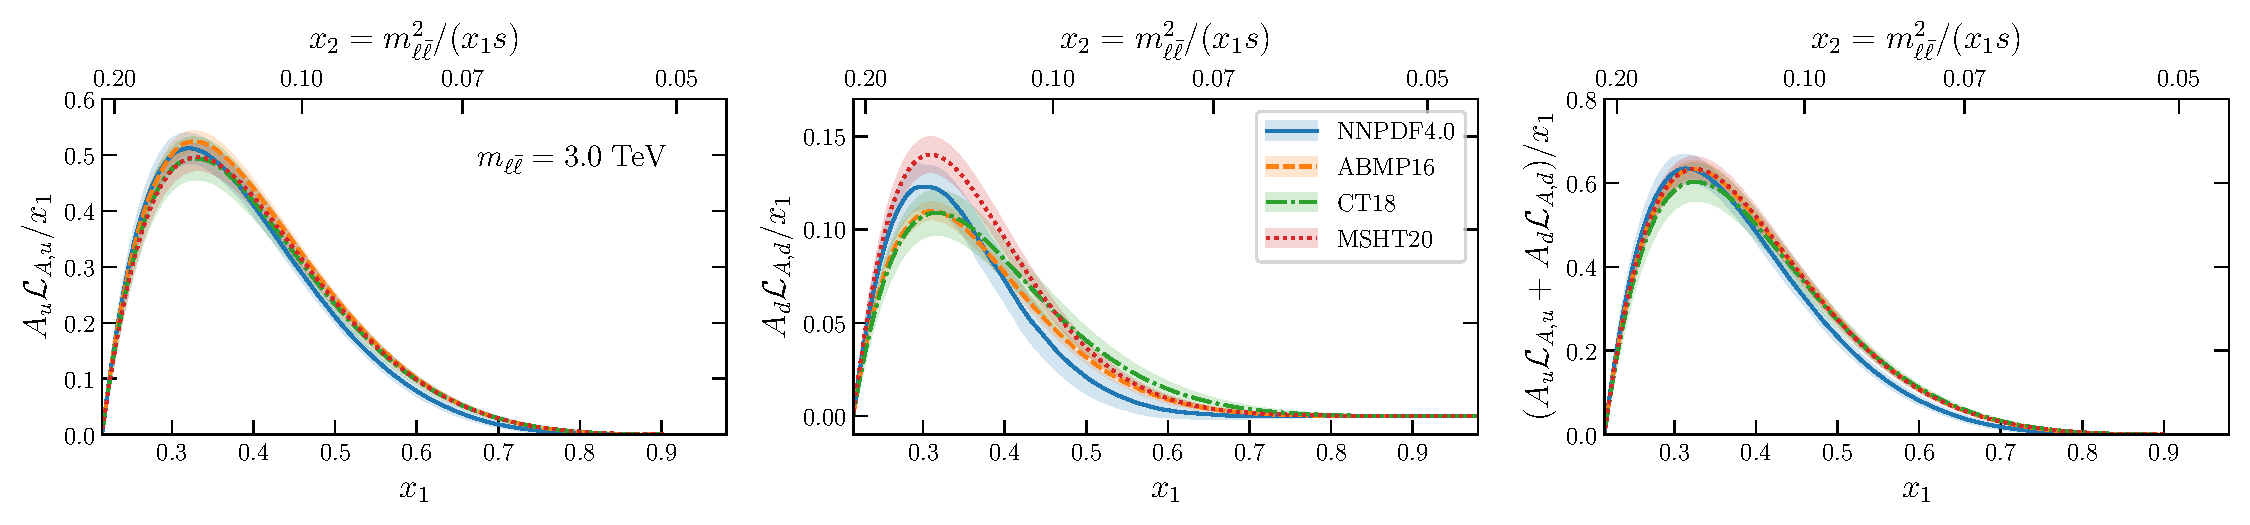
\includegraphics[width=1.00\linewidth]{ch-afb/pdfplot-abs-jacobian-DYlumis-pdfsets-minus-q3p0tev.pdf}
 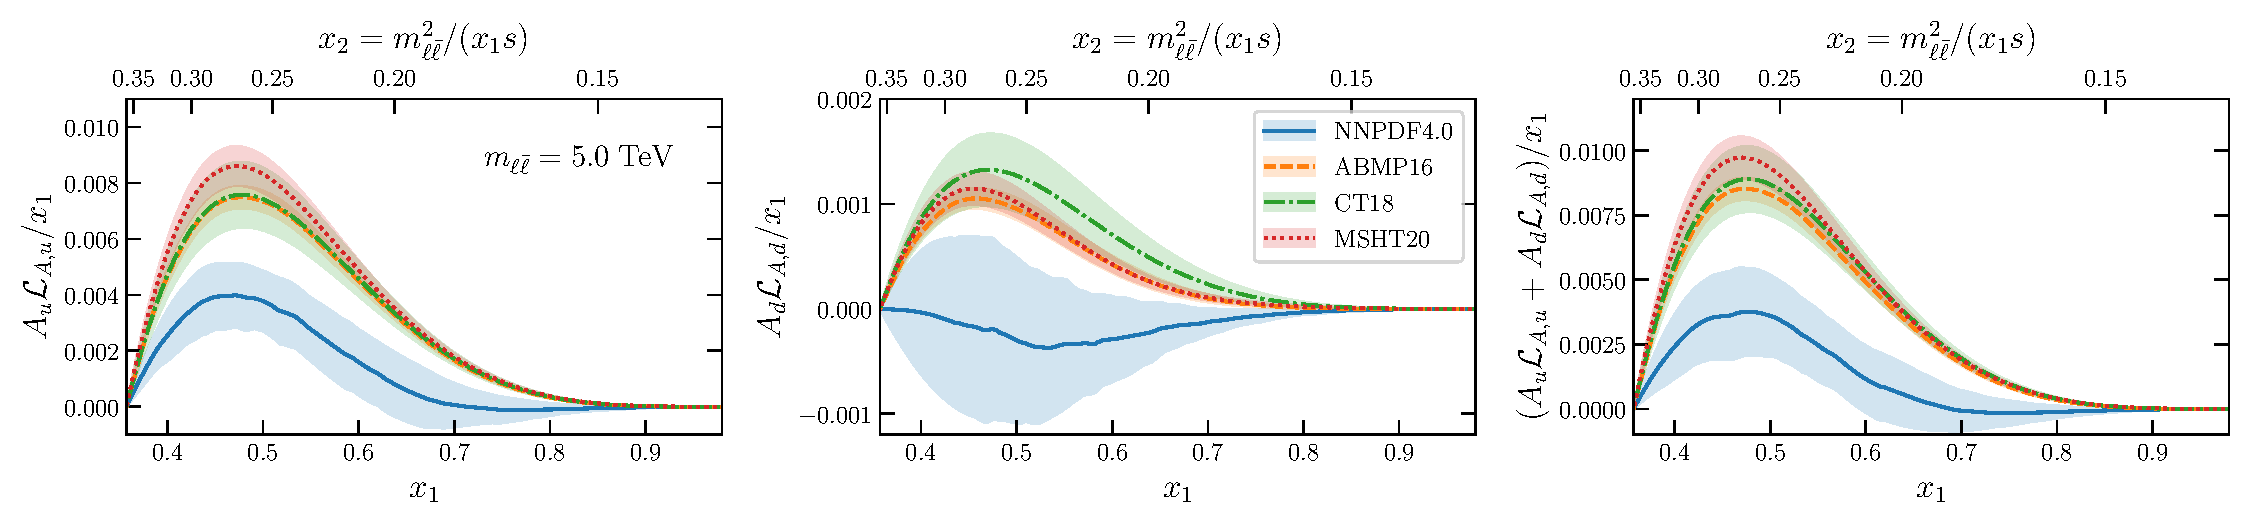
\includegraphics[width=1.00\linewidth]{ch-afb/pdfplot-abs-jacobian-DYlumis-pdfsets-minus-q5p0tev.pdf}
 \caption{The antisymmetric 
   parton luminosities $\mathcal{L}_{A,q}(x_1,\mll)$ for the \nnpdfr{4.0}, ABMP16,
   CT18, and MSHT20 \nnlo \pdf sets for dilepton
   invariant masses of
   $\mll=3$ TeV (top) and $\mll=5$ TeV (bottom).
   %
   The luminosities are multiplied by the effective charges
   $A_q$ defined in \cref{eq:afb/coup}.
   %
   From left to right, we display $\mathcal{L}_{A,u}$,  $\mathcal{L}_{A,d}$,
   and their weighted sum that enters the  coefficient $g_{A,q}$ \cref{eq:afb/gAq_integrated_1}.
    }    
 \label{fig:afb/mll_dep_lumi_minus}
\end{figure}
%---------------------------------------------------------------------------

%-------------------------------------------------------------------------------
\begin{figure}[!t]
 \centering
 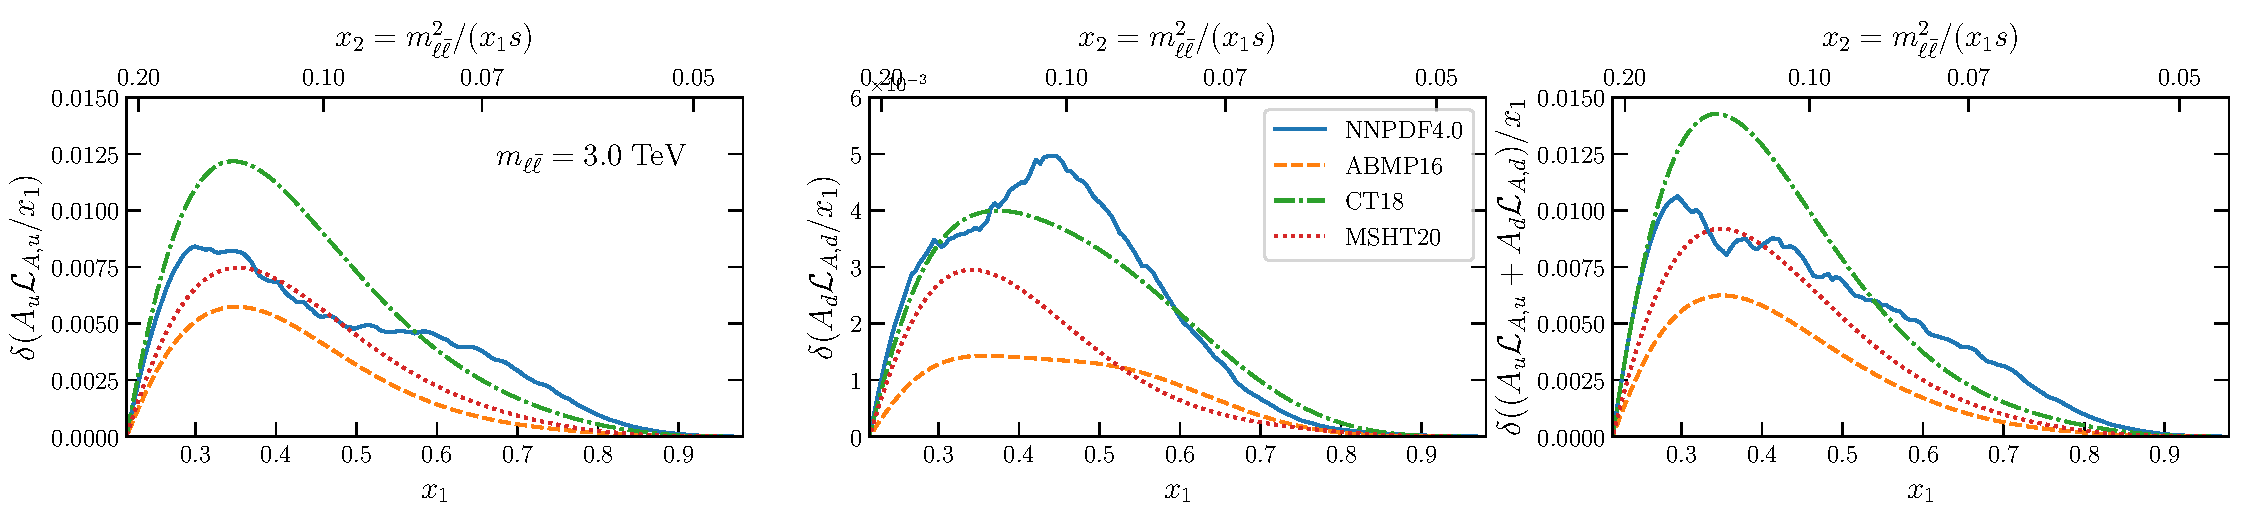
\includegraphics[width=1.00\linewidth]{ch-afb/pdfplot-abs-jacobian-DYlumis-pdfsets-minus-q3p0tev-pdferrs.pdf}
 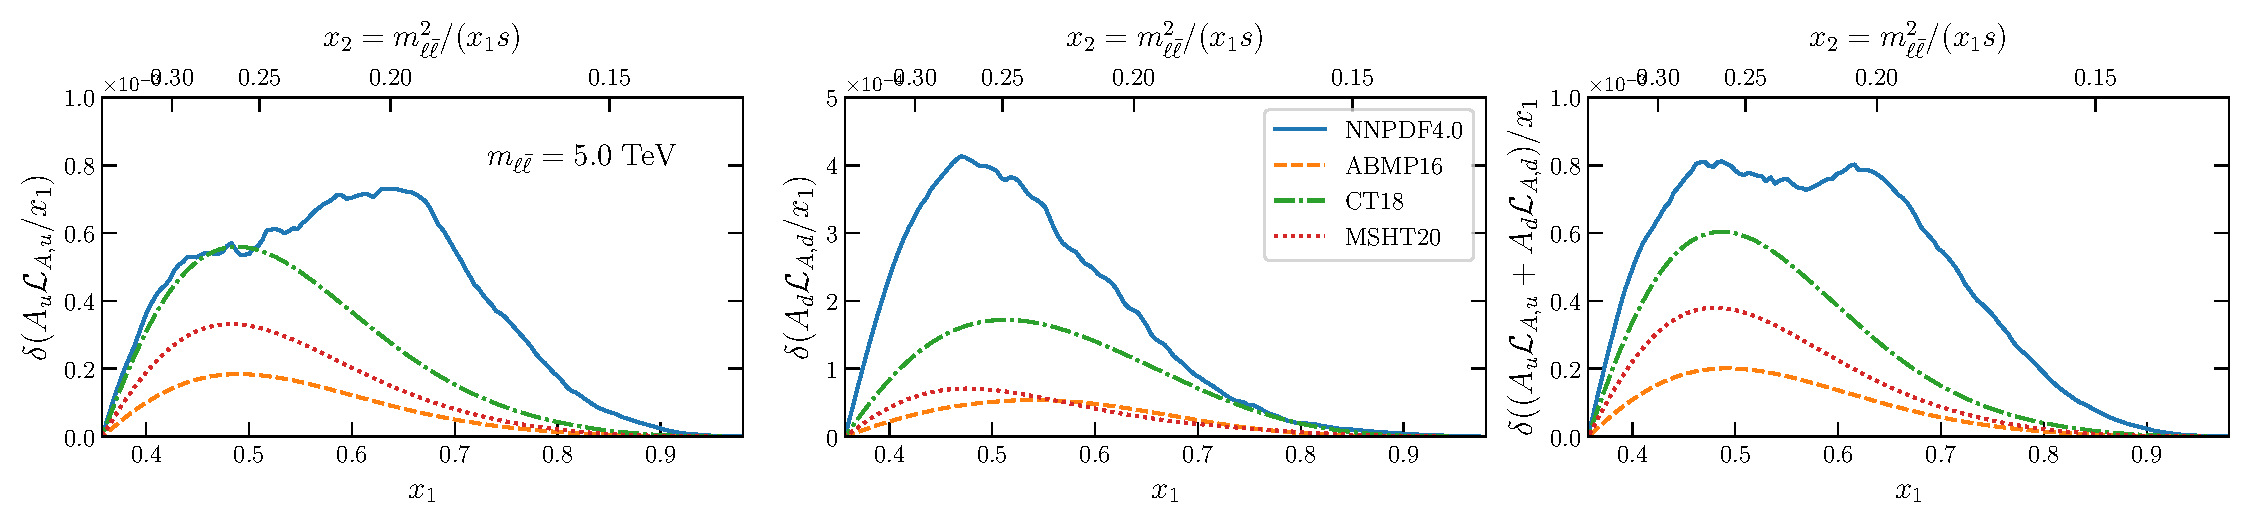
\includegraphics[width=1.00\linewidth]{ch-afb/pdfplot-abs-jacobian-DYlumis-pdfsets-minus-q5p0tev-pdferrs.pdf}
 \caption{Same as \cref{fig:afb/mll_dep_lumi_minus} now for the absolute \pdf uncertainties.
    }    
 \label{fig:afb/mll_dep_lumi_minus_pdferrs}
\end{figure}
%---------------------------------------------------------------------------

\cref{fig:afb/mll_dep_lumi_minus} shows that for ABMP16, CT18, and
MSHT20 the antisymmetric
parton luminosities depend only mildly on $\mll$, whereas for \nnpdfr{4.0}
they exhibit a strong $\mll$ dependence.
%
Indeed, for dilepton invariant masses of $\mll=3$ TeV there is good
agreement between the three groups, but
for $\mll=5$ TeV the \nnpdfr{4.0} up quark luminosity, while preserving a
similar valence-like shape, is suppressed
by a factor 2 in comparison  to other groups, and the down quark luminosity becomes compatible with zero with a negative
central value,  as already noted. 
%
For all \pdf sets and  $\mll$ values the weighted sum is dominated by the up quark contribution.
The strong scale dependence of $\mathcal{L}_{A,q}$ in \nnpdfr{4.0}
reflects the underlying \pdf behavior seen in  \cref{fig:afb/mll_dep_pdfs}
and highlighted by the effective exponents \cref{fig:afb/asy_exponents}.
%
As the scale $\mll$ increases, a range of increasingly large $x$ values is probed,
for which, in the case of
\nnpdfr{4.0}, the quark effective exponent slowly increases and the
antiquark exponent rapidly drops.
%
This leads to a negative asymmetry, 
following  \cref{eq:afb/signas}. 

A comparison of the corresponding \pdf uncertainties, displayed in
\cref{fig:afb/mll_dep_lumi_minus_pdferrs}, clearly shows the transition
from the data region to the extrapolation region.
%
For
$\mll=3$~TeV the uncertainty $\delta \mathcal{L}_{A,u}$ is generally
small for all sets, with CT18
showing a somewhat larger uncertainty for the up quark, and comparable
uncertainties for the down quark for all \pdf sets.
%
As the scale  increases to $\mll=5$~TeV, where the large-$x$ region is
probed,  the uncertainty 
increases, though more markedly for \nnpdfr{4.0}.
%
For all \pdf sets but
\nnpdfr{4.0}, the
uncertainty is approximately unchanged when the scale is further increased,
while for \nnpdfr{4.0} it grows markedly.

Finally, in \cref{fig:afb/asym_coeff_mlldep} we display for all
\pdf sets the
ratio of antisymmetric to symmetric couplings
\begin{equation}
\label{eq:afb/coupling_ratio}
R_{\text{fb}}\equiv \frac{\sum_q g_{A,q}}{\sum_{q'} g_{S,{q'}}} \, ,
\end{equation}
that, according to
\cref{eq:afb/afb_lo}, determines at leading order
the sign and magnitude
of the forward-backward asymmetry distribution $A_{\text{fb}}(\cos\theta^*)$.
%
The symmetric and antisymmetric coefficients are obtained by integrating
the corresponding symmetric $\mathcal{L}_{S,q}$ and antisymmetric
$\mathcal{L}_{A,q}$ partonic luminosities according to
\cref{eq:afb/gAq_integrated_1}, and the result is shown as a function of the lower integration cut $\mll^{\text{min}}$.
%
In all cases the correlation between \pdf uncertainties in the numerator and
the denominator are kept into account.

%-------------------------------------------------------------------------------
\begin{figure}[!t]
 \centering
 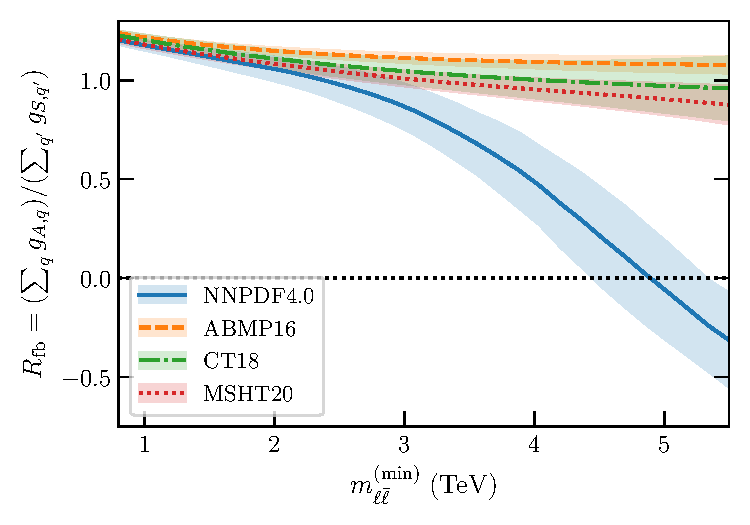
\includegraphics[width=0.60\linewidth]{ch-afb/asym_coeff_mlldep.pdf}
 \caption{
   The coupling ratio $R_{\text{fb}}$, \cref{eq:afb/coupling_ratio}, that
   enters the forward-backward asymmetry $A_{\text{fb}}(\cos\theta^*)$ at \lo, 
   \cref{eq:afb/afb_lo}, for different \pdf sets, as  a function of the lower
   cut in the dilepton invariant mass $\mll^{\text{min}}$.
 }    
 \label{fig:afb/asym_coeff_mlldep}
\end{figure}
%---------------------------------------------------------------------------

\cref{fig:afb/asym_coeff_mlldep} shows that, consistently
with the behavior of the luminosity of
\cref{fig:afb/mll_dep_lumi_minus},  for $\mll^{{\rm
    min}}\lsim 3$~TeV results agree within uncertainties for all \pdf
sets.
%
The situation is different for higher dilepton invariant masses $\mll^{{\text{min}}}\gsim 3$~TeV:
the ratio $R_{\text{fb}}$ starts to decrease for \nnpdfr{4.0}, while it
remains approximately  constant 
for the other  \pdf sets. In particular, for \nnpdfr{4.0} the coupling ratio
vanishes around $\mll^{{\text{min}}}\sim5$~TeV, and it becomes negative
for yet larger   $\mll^{{\text{min}}}$ values.
It follows that the forward-backward
asymmetry in high-mass Drell-Yan production should decrease  and
eventually vanish (and possibly even turn negative)
in \nnpdfr{4.0} as the $\mll^{{\text{min}}}$ cut is increased,
while for CT18, MSHT20, and ABMP16 it should remain positive
with a similar magnitude irrespective of the cut  $\mll^{{\text{min}}}$ adopted.

%-------------------------------------------------------------------------------
\begin{figure}[!t]
 \centering
 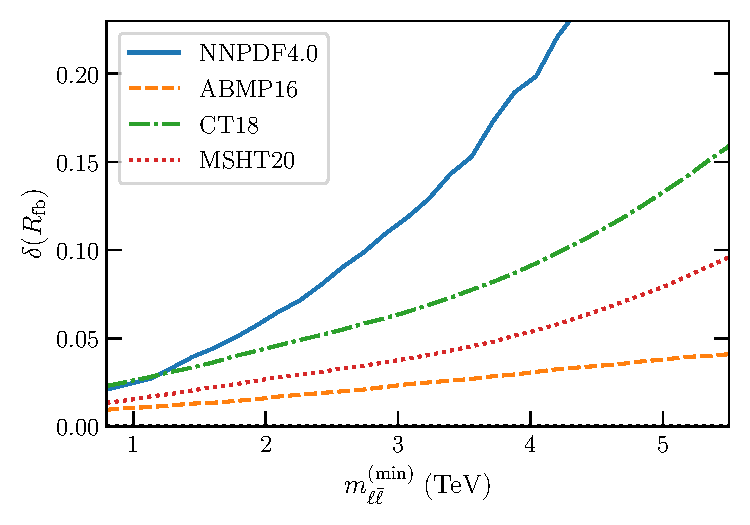
\includegraphics[width=0.49\linewidth]{ch-afb/asym_coeff_mlldep_abserr.pdf}
 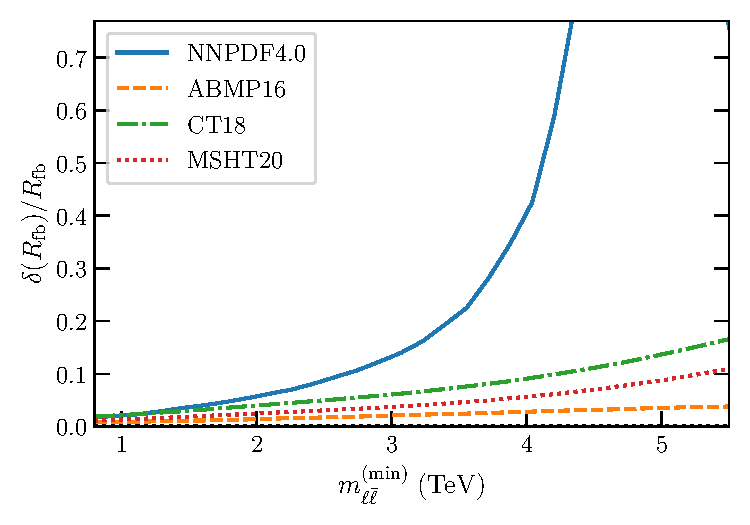
\includegraphics[width=0.49\linewidth]{ch-afb/asym_coeff_mlldep_relerr.pdf}
 \caption{The absolute (left) and relative (right panel) uncertainties
   in the coupling ratio $R_{\text{fb}}$ shown in \cref{fig:afb/asym_coeff_mlldep}.
 }    
 \label{fig:afb/asym_coeff_mlldep_err}
\end{figure}
%---------------------------------------------------------------------------

\cref{fig:afb/asym_coeff_mlldep_err} displays the 
absolute  and relative  uncertainties
associated to the coupling ratio $R_{\text{fb}}$.
%
We observe that \nnpdfr{4.0} shows
the most marked increase of the uncertainties in $R_{\text{fb}}$
as $\mll^{\text{min}}$ grows.
%
For instance, for  $\mll^{\text{min}}\gtrsim4$~TeV
the absolute \pdf uncertainty in \nnpdfr{4.0}
is about twice as large as that found using CT18 
four times as large as MSHT20,
and about one order of magnitude larger than ABMP16.
%
This trend is magnified for the relative uncertainties
due to the decrease in the central value of $R_{\text{fb}}$
as $\mll^{\text{min}}$ increases.
